\section*{Analysis}
\label{sec:analysis}

The emulator is used to perform the debugging (although it does not seem to be able to run RenderScript code).
To run the code, we are using two devices for the analysis.
The first is a Nexus 7 with the following specs:

\begin{verbatim}
    CPU: Qualcomm Snapdragon S4 Pro, 1.5GHz
    GPU: Adreno 320, 400MHz
    Memory - 2 GB
    Storage 32 GB
\end{verbatim}

The second is a Samsung Galaxy Nexus with the following specs:

\begin{verbatim}
    CPU: ARMv7, 2 cores, 1200 Mhz, SIMD NEON
    Memory: 694, JVM max: 96 MB
    GPU: PowerVR SGX 540.
\end{verbatim}


\subsection*{Preliminary Results}

While we do have implementations for 3 out of the 4 benchmarks we promised in the proposal schedule,
  our results only show part of those.
The data has not been fully analyzed, but we can give some preliminary insights into the expected
  results.

The IO times are around 1000 times more than the compute times on Android devices.
Therefore, in the plots we chose not to include the IO times, since that heavily skews
  the plots, and using a log scale it makes the other data almost the same.

The plots record the time it took to allocate the data (which should be similar across implementations),
  the compute time, and for RenderScript the setup time --- this is the time it takes to load the RenderScript code as you prepare for computation (it may include jitting the code for example).

Vector addition, shown in figure~\ref{fig:vecadd}, is a simple kernel and we see that the serial version outperforms both RenderScript
  and the threaded Java version.
For the RenderScript, we suspect this is overhead from translating between the Java data arrays and
  the RenderScript arrays.
For the threaded version, we use a thread for each element calculation (in the same style as you'd do in CUDA), and therefore you result in huge runtime penalty because of launching many threads.
Performing thread coarsening would decrease this impact, but that has not been done. 

\begin{figure}[t!]
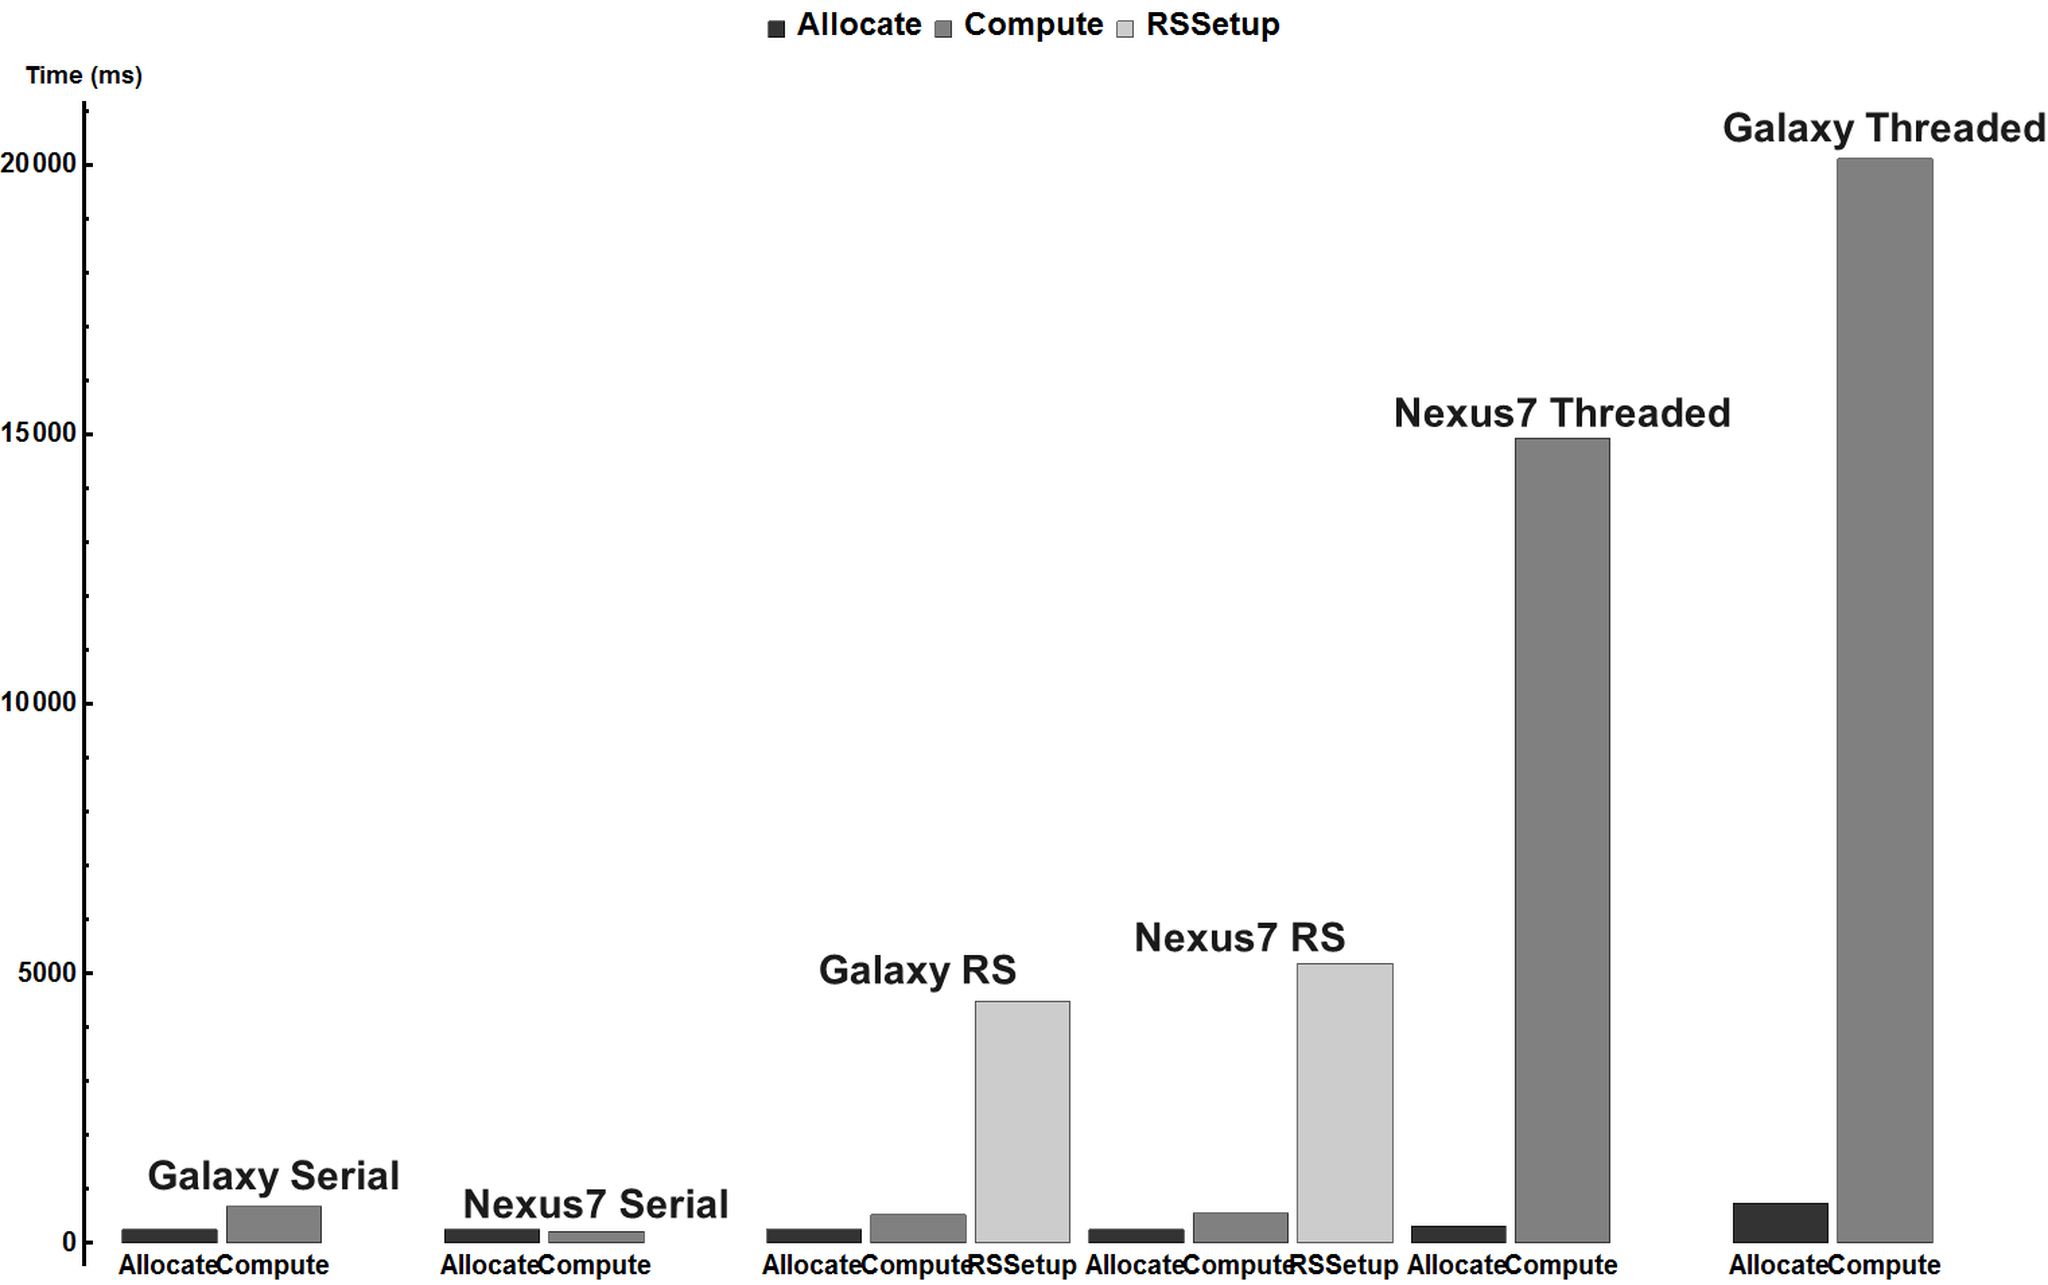
\includegraphics[scale=0.125]{VectorAdd_nolog.png}
\caption{VectorAdd Benchmark.}
\label{fig:vecadd}
\centering
\end{figure}

The large RenderScript setup time might either be because this benchmark does not take too much time
  to run and therefore the difference is apparent, or because it is the first benchmark we run and
  the RenderScript initial load time is added.
Further investigation is required, but in general we plan on extending our benchmark framework so 
  it performs multiple runs, discarded the time for the first run, and computes the mean time.



Matrix multiplication, shown in figure~\ref{fig:sgemm}, performs matrix multiplication.
The data is stored in column major order and we perform the computation in column major order.
One possible optimization is to transpose the data beforehand to get better locality when performing computation.
Regardless, we see a 4x performance improvement in SGEMM.
We have not implemented a threaded Java version of the SGEMM benchmark, which is why it's missing from
  the plot.
\begin{figure}[t!]
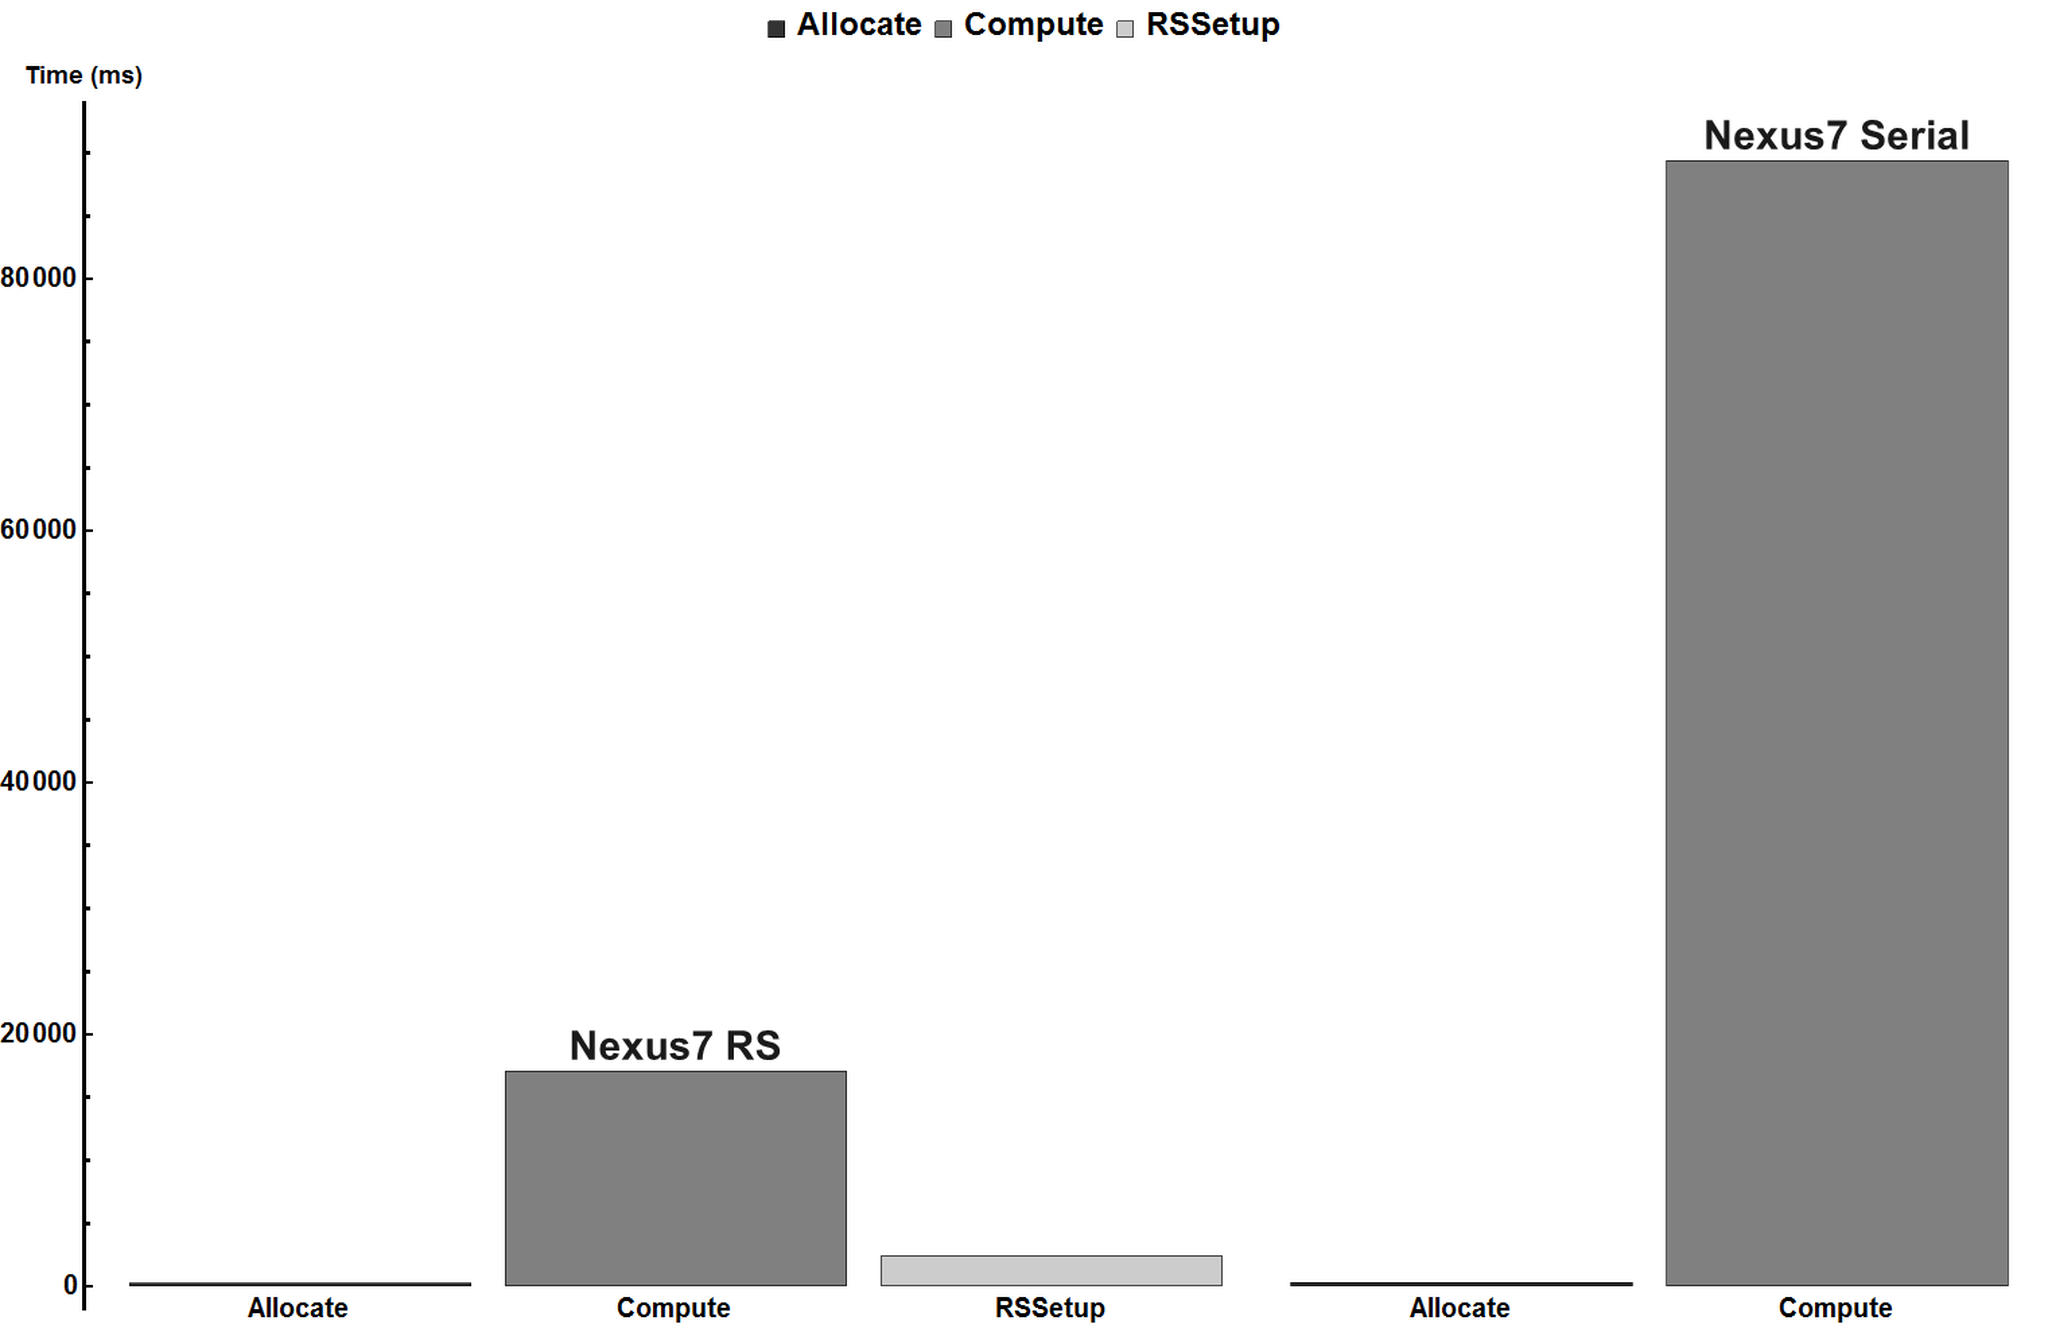
\includegraphics[scale=0.125]{Sgemm_nolog.png}
\caption{Matrix Matrix Multiplication Benchmark.}
\label{fig:sgemm}
\centering
\end{figure}


Note, the semantics of Java's single precision floating point operations are slightly different from those of C, so do not expect 
  to always use single precision for all the benchmarks (this was seen in the initial porting of TPACF).



The final benchmark implemented is stencil shown in figure~\ref{fig:stencil}.
Again, we did not implement the threaded Java version of this code, but we can see that the 
  RenderScript version outperforms the serial code.
RenderScript has not scratch pad memory constructs, so we were not able to use fine grained memory management to achieve high throughput.
We further suspect that this code is not fully optimized to use all the RenderScript constructs available.
Finally, the serial versions have an added (negligible) {\tt RSSetup} time, this is either due to bad parsing of the 
  output data or an incorrect labeling of a timer in the source code.

\begin{figure}[t!]
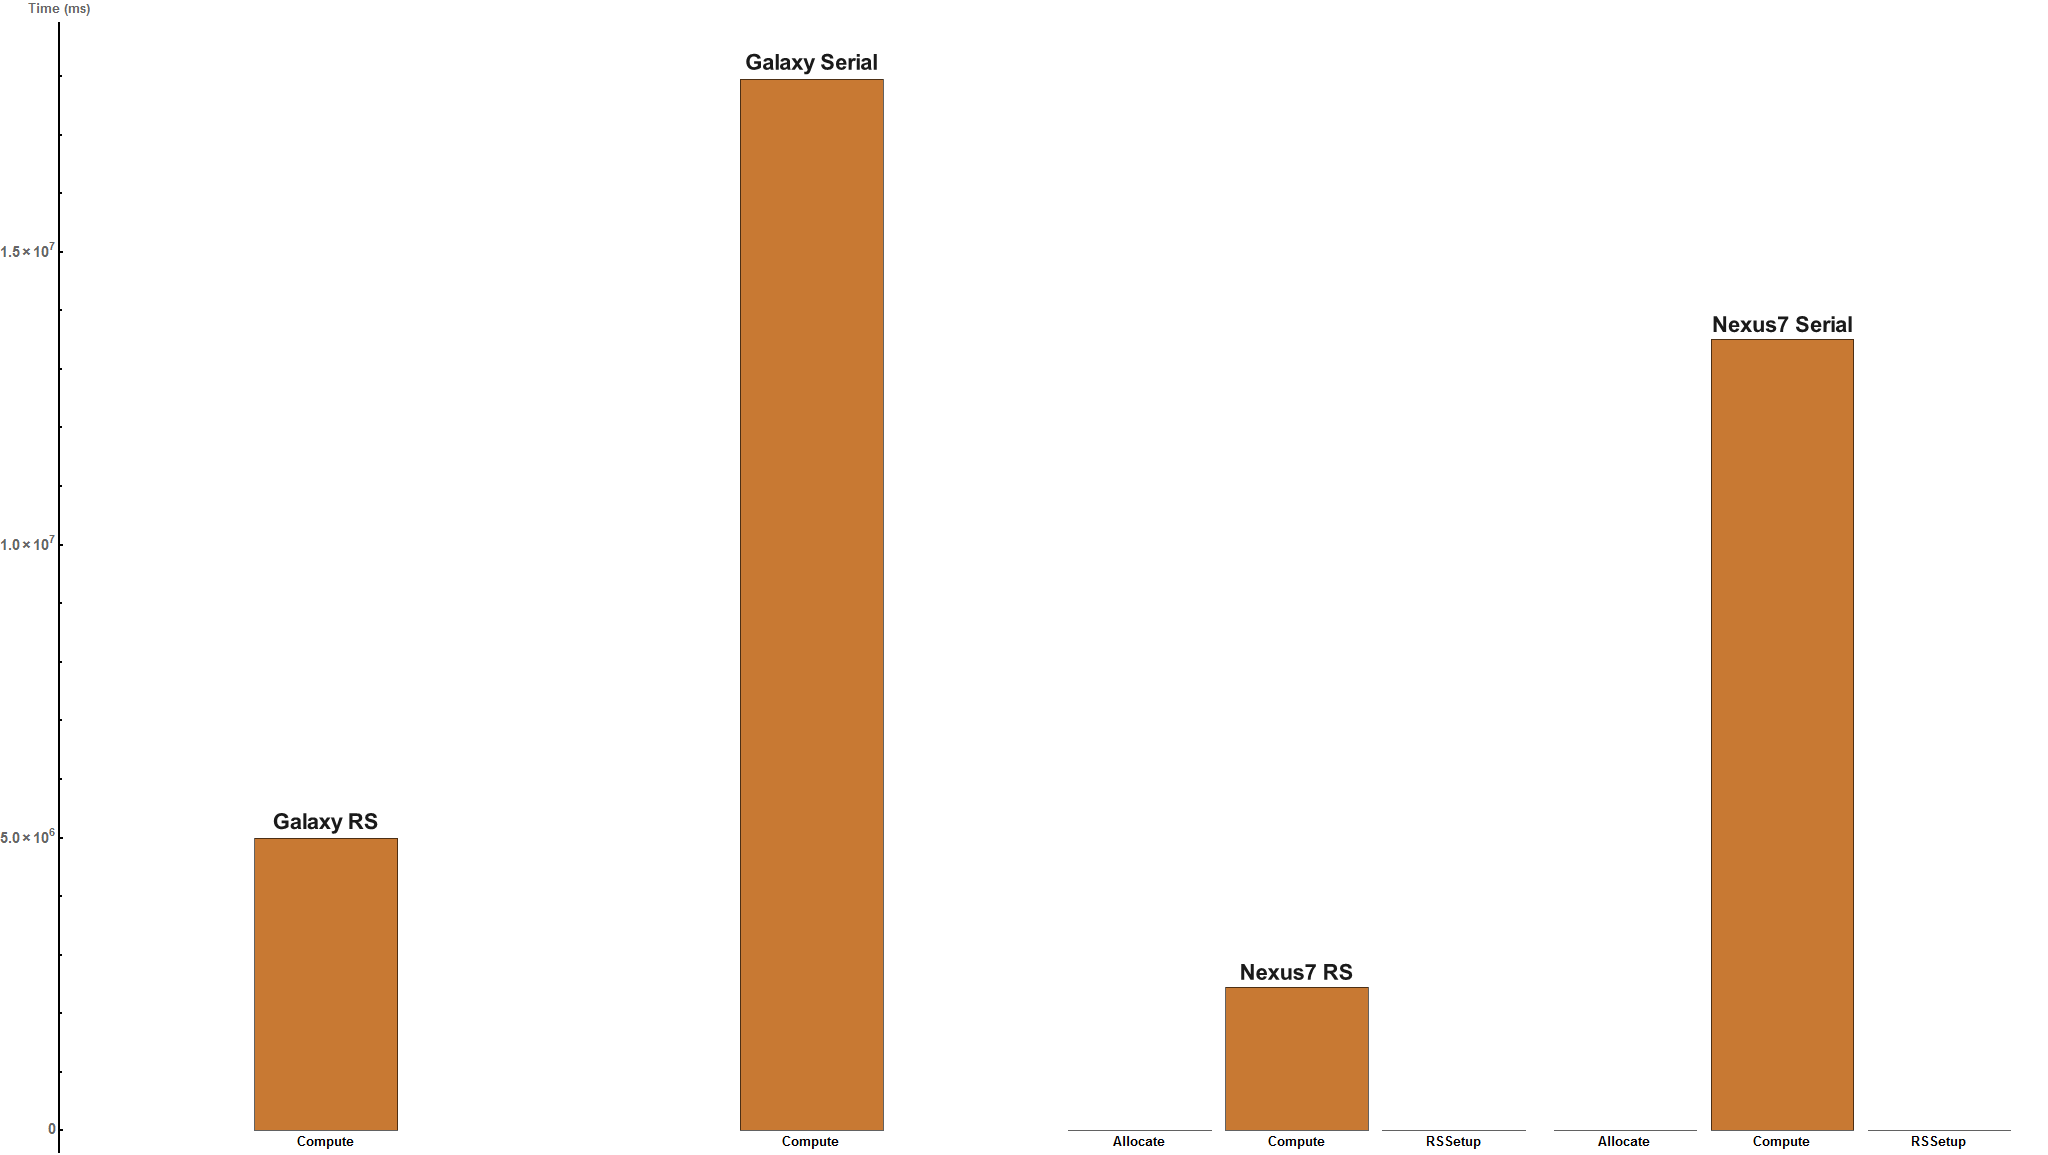
\includegraphics[scale=0.125]{Stencil_nolog.png}
\caption{Stencil Benchmark.}
\label{fig:stencil}
\centering
\end{figure}


  

